\setcounter{chapter}{10}

\chapter{重积分({\it 及其应用})}

{\it (多)重积分就是多元函数的积分,就好像多重极限就是多元函数的极限一样}

\begin{description}
	\item[{\bf 二重积分:}] 
		$$\iint_Df(x,y)\d\sigma$$ 
	\item[{\bf 三重积分:}] 
		$$\iiint_{\Omega}f(x,y,z)\d V$$ 
\end{description}

{\bf Keyword:}积分区域、被积函数、面积(体积)微元

\section{概念与性质}

{\bf Insight:}{\it “分割取近似,做和求极限”}

{\bf P176-例:}求立体体积
$$\Omega:0\leq x\leq 1,0\leq y\leq 1,0\leq z\leq 3-x^2-y^2$$

\begin{center}
	\resizebox{!}{4.2cm}{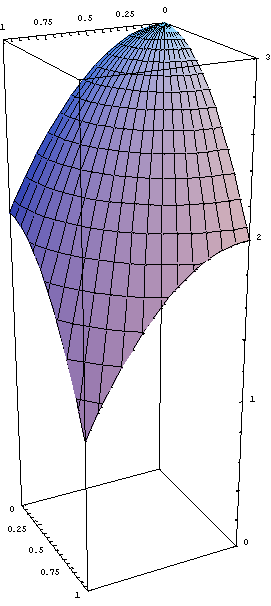
\includegraphics{./images/ch11/volO.pdf}}\quad 
	\resizebox{!}{4.2cm}{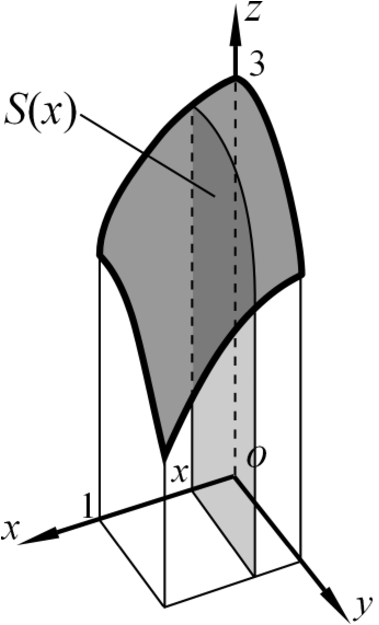
\includegraphics{./images/ch11/volD.pdf}}\quad 
	\resizebox{!}{4.2cm}{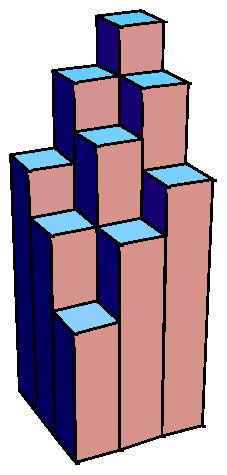
\includegraphics{./images/ch11/volC.pdf}}\quad 
	\resizebox{!}{4.2cm}{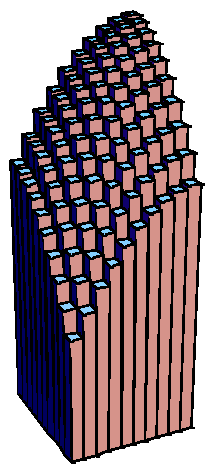
\includegraphics{./images/ch11/volX.pdf}}
\end{center}

{\bf 微元法:}体积微元
$$dV=S(x)dx$$
截面积:
$$S(x)=\dint_0^1(3-x^2-y^2)dy=\df 83-x^2$$
$$V=\dint_0^1S(x)dx=\df 73$$

{\bf 例}(立体的质量)设以上$\Omega$内部任一点$(x,y,z)$处的密度为$\rho=1+z$,
求$\Omega$的质量。

{\bf 微元法:}体积微元
$$dV=S(x)dx$$
截面积:
$$S(x)=\dint_0^1(3-x^2-y^2)dy=\df 83-x^2$$
$$V=\dint_0^1S(x)dx=\df 73$$

{\bf 定义:}
\begin{enumerate}[(1)]
  \setlength{\itemindent}{1cm}
  \item {\bf 二重积分:} 
  $$\iint_Df(x,y)\d\sigma=\lim_{d(T)\to
  0}\sum_{i=1}^nf(\xi_i,\eta_i)\Delta\sigma_i$$ 
  \item {\bf 三重积分:} 
  $$\iiint_{\Omega}f(x,y,z)\d V=\lim_{d(T)\to
  0}\sum_{i=1}^nf(\xi_i,\eta_i,\zeta_i)\Delta V_i$$
\end{enumerate}

{\bf 基本性质:}
\begin{enumerate}[(1)]
  \setlength{\itemindent}{1cm}
  \item {\bf 线性性} 
  \item {\bf 区域可加性} 
  \item {\bf 保号性I:} 若在$D$上,$f(x,y)\geq 0$,则
  $$\iint_Df(x,y)\d\sigma\geq 0$$ 
  \item {\bf 保号性II:} 若$f(x,y)$在$D$上连续,则
  $$\iint_Df(x,y)\d\sigma=0$$
  当且仅当在$D$上恒有$f(x,y)=0$
    \begin{itemize}
	  \item 若在$D$上,$f(x,y)\leq g(x,y)$,则
	  $$\iint_Df(x,y)\d\sigma\leq\iint_Dg(x,y)\d\sigma$$ 
	  \item $$\left|\iint_Df(x,y)\d\sigma\right|\leq\iint_D|f(x,y)|\d\sigma$$ 
	  \item 设$M,m$分别为$f(x,y)$在$D$上的最大和最小值,$D$的面积为$A$,则
	  $$mA\leq\iint_Df(x,y)\d\sigma\leq MA$$
	\end{itemize}
  \item {\bf 积分中值定理:}设函数$f(x,y)$在有界闭区域$D$上连续非负,$D$的面积为$A$,则存在
	$(\xi,\eta)\in D$,使得
	$$\iint_Df(x,y)\d\sigma=f(\xi,\eta)A$$
\end{enumerate}

{\bf 注:通过与定积分的类比,理解、记忆重积分的概念与性质}

\section{重积分的计算}

{\bf Keyword:}积分次序

\subsection{二重积分}

$${\iint_Df(x,y)\d\sigma=\lim_{d(T)\to
  0}\sum_{i=1}^nf(\xi_i,\eta_i)\Delta\sigma_i}$$
 令$\d\sigma=\d y\d x$\ps{相当于对积分区域进行水平和竖直的分割}, 且
$$D=\{x_1\leq x\leq x_2,\varphi_1(x)\leq y\leq \varphi_2(x)\}$$
 则二重积分可化为{\bf 累次积分:}
$${\iint_Df(x,y)\d\sigma=\int_{x_1}^{x_2}
\int_{\varphi_1(x)}^{\varphi_2(x)}f(x,y)\d y\d x}$$

{\bf 计算步骤:}

\begin{enumerate}
  \setlength{\itemindent}{1cm}
  \item {\bf 画图:}描绘积分区域$D$的图形 
  \item {\bf 定限:}确定累次积分的积分限 
  \item {\bf 求积分:}依次计算累次积分的值 
\end{enumerate}

{\bf 积分区域与累次积分的次序:}
将二重积分化为累次积分时,不同的积分次序,对应于不同的积分区域表示方法

{\bf P187-例1:}计算
$$\iint_Dxy\d\sigma,$$
其中$D$为抛物线$y=x^2$和$x=y^2$所围区域。

\begin{itemize}
  \item {先$x$后$y$:}$D:y^2\leq x\leq\sqrt y,\,0\leq y\leq 1$ 
  \item {先$y$后$x$:}$D:x^2\leq y\leq\sqrt x,\,0\leq x\leq 1$
\end{itemize}

{\bf P187-例2:}计算
$$\iint_D\df{x^2}{y^2}\d\sigma,$$
其中$D$由直线$y=2,\,y=x$和$xy=1$围成。

{\bf 注:}合理选择积分次序,简化累次积分的计算

{\bf P188-例3:}计算
$$\iint_D\df{\sin y}{y}\d\sigma,$$
其中$D$由$x=y^2$和$y=x$所围成。

{\bf P190-例5:}计算累次积分
$$I=\int_{1/4}^{1/2}\int_{1/2}^{\sqrt y}e^{y/x}\d x\d y+
\int_{1/2}^1\int_y^{\sqrt y}e^{y/x}\d x\d y$$

{\bf P189-例4:}求两柱面$x^2+y^2=R^2,\, x^2+z^2=R^2$
相交所围成的立体体积。

\begin{center}
	\resizebox{!}{5cm}{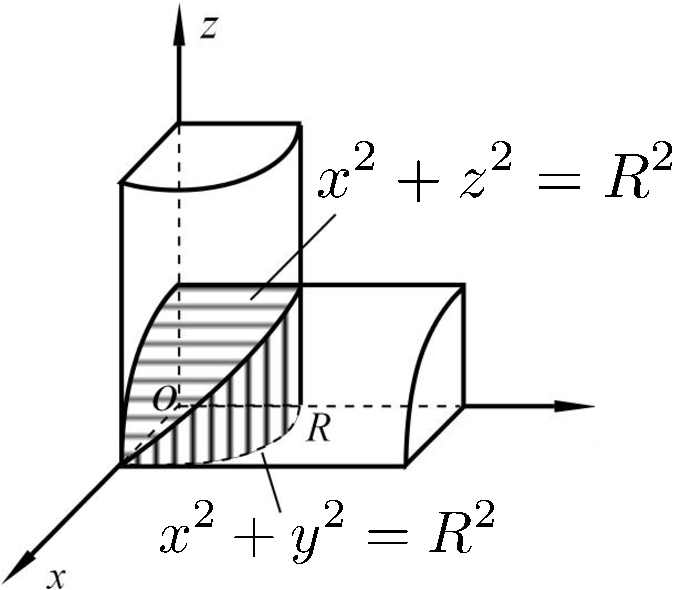
\includegraphics{./images/ch11/intersectV.pdf}}
\end{center}

\subsection{三重积分}

$${I=\iiint_{\Omega}f(x,y,z)\d V}$$
\begin{enumerate}
  \item {\bf 微元法(投影法):}
  $$I=\iint_D\int_{z_1(x,y)}^{z_2(x,y)}f(x,y,z)\d z\d\sigma$$
  \item {\bf 截面法:}
  $$I=\int_{z_1}^{z_2}\iint_{D(z)}f(x,y,z)\d\sigma \d z$$
\end{enumerate}

\subsubsection{微元法(投影法)}

设$\Omega$在$xOy$平面上的投影区域为$D$, $\d V=\d z\d\sigma$, \ps{先投影,再定$z$}
$$\Omega=\{z_1(x,y)\leq z\leq z_2(x,y), (x,y)\in D\}$$

\begin{center}
	\resizebox{!}{4.5cm}{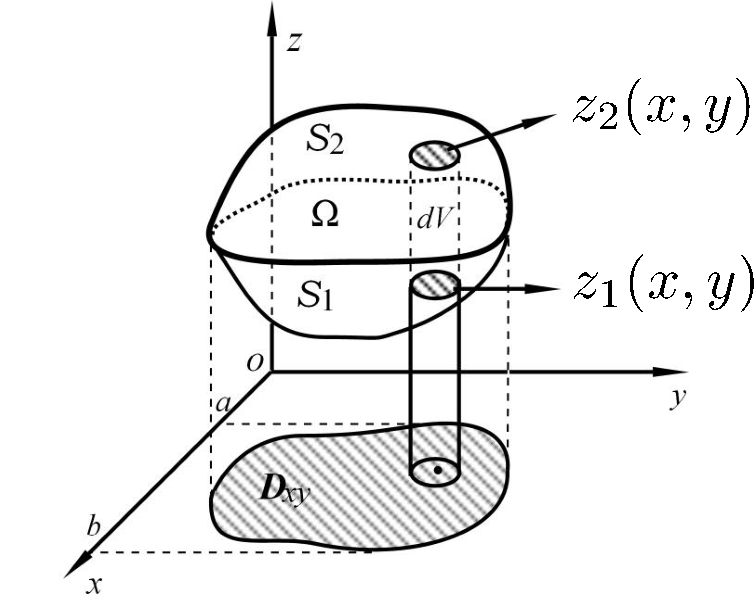
\includegraphics{./images/ch11/DxyZ.pdf}} 
\end{center}

$${I=\iiint_{\Omega}f(x,y,z)\d
V=\iint_D\int_{z_1(x,y)}^{z_2(x,y)}f(x,y,z)\d z\d\sigma}$$

{\bf P193-例7:}计算三重积分
$$I=\iiint_{\Omega}\df 1{(1+x+y+z)^3}\d V,$$
其中$\Omega$为平面$x+y+z=1$与三个坐标面所围成的空间区域。

\subsubsection{截面法}

取$\Omega$的水平截面,其在$xOy$平面上的投影区域为$D(z)$,
$\d V=\d\sigma \d z$,\ps{先定$z$,再投影}
$$\Omega=\{(x,y)\in D(z),z_1\leq z\leq z_2\}$$

\begin{center}
	\resizebox{!}{4.5cm}{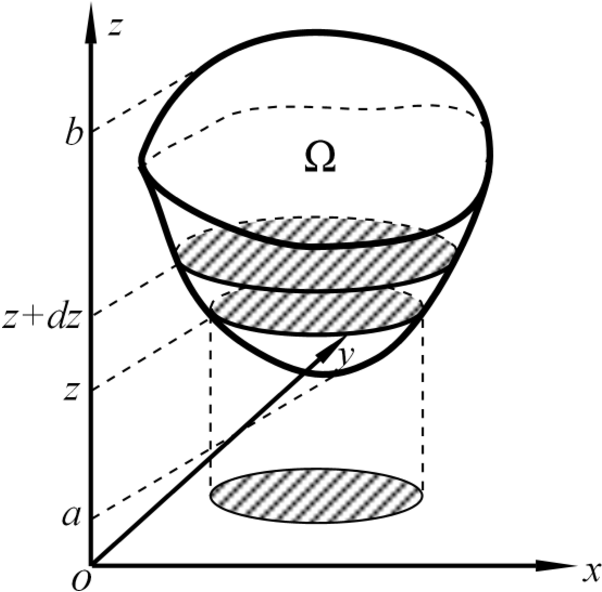
\includegraphics{./images/ch11/Dzxy.pdf}}
\end{center}

$${I=\iiint_{\Omega}f(x,y,z)\d
V=\int_{z_1}^{z_2}\iint_{D(z)}f(x,y,z)\d\sigma \d z}$$

{\bf 例:}计算三重积分
$$I=\iiint_{\Omega}z^2\d V,$$
其中$\Omega:\df{x^2}{a^2}+\df{y^2}{b^2}+\df{z^2}{c^2}\leq 1$。

{\bf 注:}如果被积函数只与$z$有关,用截面法会比较容易计算。

{\bf P194-例8:}将三重积分
$$I=\iiint_{\Omega}f(x,y,z)\d V,$$
化为累次积分,其中$\Omega$为曲面$z=1-x,y=1-z^2$及三个坐标平面所围空间闭区域。

{\bf P195-例9:}计算三重积分
$$I=\iiint_{\Omega}(x+y+2z)\d V,$$
其中$\Omega$为球体$x^2+y^2+z^2\leq R^2\,(R>0)$在第一卦限中的部分。

{\bf 思考题:}讨论数列$a_n=\ds\iiint_{\Omega_n}z^n\d V$的敛散性,其中
$\Omega_n$由$(x^2+y^2+z^2)^n=a^{2n-1}z\;(a>0)$所围。\hfill $a\in(0,1]$收敛;
反之发散。

\section{坐标变换与重积分的计算}

{\bf Keyword:}坐标变换、Jacobi行列式

\subsection{二重积分与极坐标}

{\bf 思考:}极坐标系下的“矩形”有哪些可能的形状?

$$I=\iint_Df(x,y)\d\sigma=\iint_Df(x,y)\d x\d y$$
在极坐标系下,面积微元${\d\sigma=\rho \d\rho \d\theta}$, 
从而
$${I=\iint_Df(x,y)\d\sigma=\iint_Df(\rho\cos\theta,\rho\sin\theta)
\rho \d\rho \d\theta}$$
{\bf 注意:}微元形式的改变意味着积分区域表示方式的变化

\begin{center}
	\resizebox{!}{4.2cm}{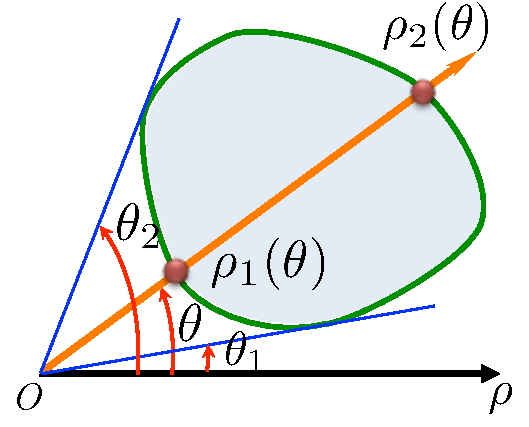
\includegraphics{./images/ch11/tr.pdf}}\hspace{2cm}
	\resizebox{!}{4.2cm}{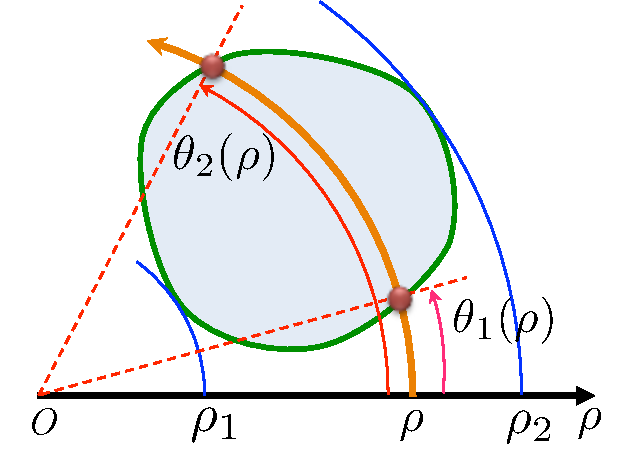
\includegraphics{./images/ch11/rt.pdf}}
	
	$D:\theta_1\leq\theta\leq\theta_2,\rho_1(\theta)\leq\rho\leq\rho_2(\theta)$
	\hspace{2cm}
	$D:\rho_1\leq\rho\leq\rho_2,\theta_1(\rho)\leq\theta\leq\theta_2(\rho)$
\end{center}

{\bf 例:}计算二重积分
$$\iint_D(x^2+y^2)\d x\d y,$$
其中$D$由圆$x^2+y^2=2y,\,x^2+y^2=4y$及直线
$x=\sqrt 3y,\,y=\sqrt 3x$围成。

{\bf P202-例1:}计算二重积分
$$\iint_D\arctan\df yx\d\sigma,$$
其中$D$为双扭线
$$(x^2+y^2)^2=a^2(x^2-y^2)\;(a>0)$$
与$x$轴正向围成图形在第一象限中的部分。

{\bf 例:}求球体$x^2+y^2+z^2\leq 4a^2$包含在圆柱$x^2+y^2=2ax\,(a>0)$
内的体积。

\begin{center}
	\resizebox{!}{5cm}{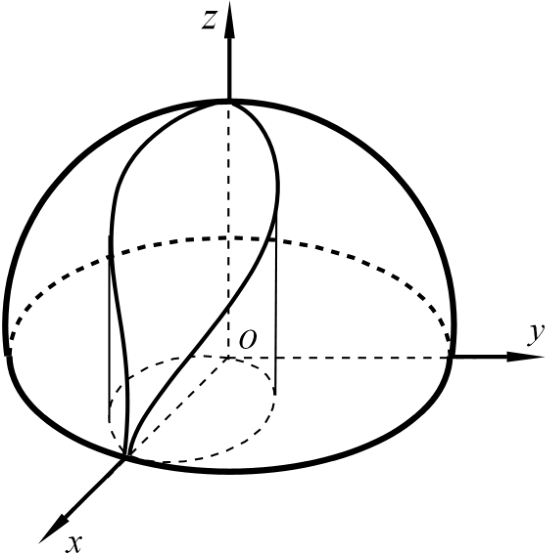
\includegraphics{./images/ch10/viviani.pdf}}
\end{center}

{\bf P203-例2:}计算椭圆抛物面$z=x^2+2y^2$与抛物柱面$z=2-x^2$所围成
的立体体积。

\begin{center}
	\resizebox{!}{5cm}{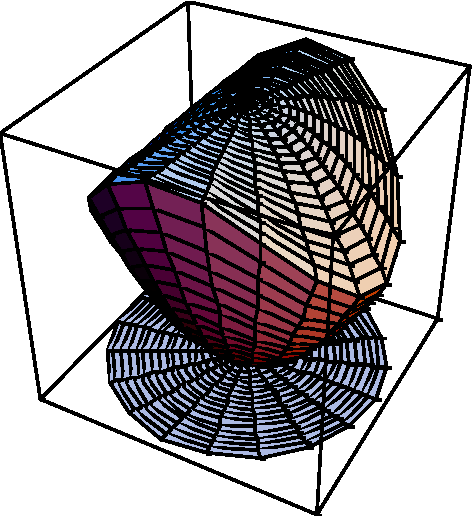
\includegraphics{./images/ch11/ub.pdf}}
\end{center}

{\bf P204-例4:}计算
$$\iint_De^{-x^2-y^2}\d x\d y,$$
其中$D:x^2+y^2\leq a^2$。利用该计算结果求
$$\dint_{-\infty}^{+\infty}e^{-x^2}\d x.$$

\subsection{三重积分与柱坐标}

{\bf 从直角坐标到柱坐标:}$M:\;(x,y,z)\;\to(\rho,\theta,z)$,其中
$$x=\rho\cos\theta,\;y=\rho\sin\theta,\;z=z\quad (\rho\geq 0,0\leq\theta\leq
2\pi,z\in\mathbb{R})$$

\begin{center}
	\resizebox{!}{5cm}{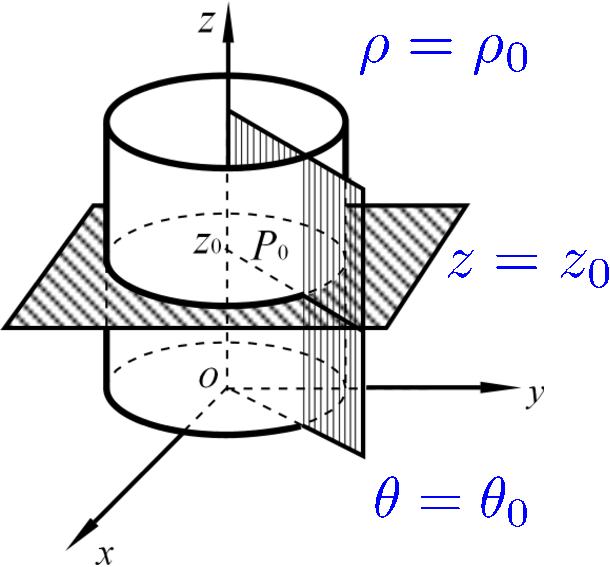
\includegraphics{./images/ch11/bucket.pdf}}
\end{center}

柱坐标系下的体积微元

\begin{center}
	\resizebox{!}{5cm}{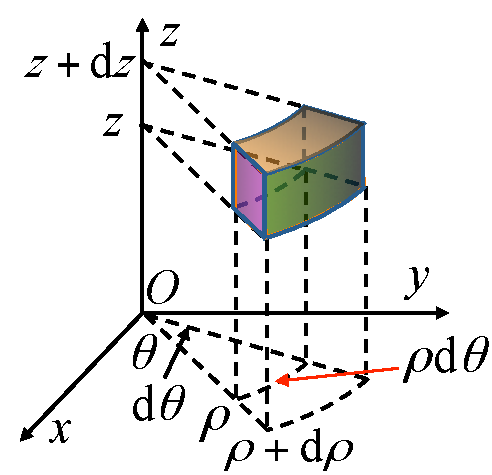
\includegraphics{./images/ch11/polarCy.pdf}}
	$$\d V=\rho \d\rho \d\theta \d z$$
\end{center}

$${\iiint_{\Omega}f(x,y,z)\d
V=\iiint_{\Omega}f(\rho\cos\theta,\rho\sin\theta,z)\rho 
\d\rho \d\theta \d z}$$

微元的表示(微元法)

\begin{center}
	\resizebox{!}{6cm}{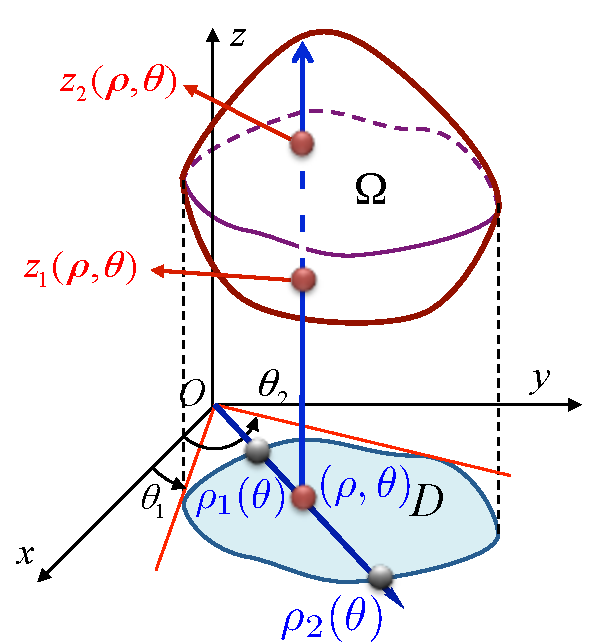
\includegraphics{./images/ch11/cy21.pdf}}
\end{center}

$$\theta_1\leq\theta\leq\theta_2,\;
\rho_1(\theta)\leq\rho\leq\rho_2(\theta),\;
z_1(\rho,\theta)\leq z\leq z_2(\rho,\theta)$$

{\bf P209-例6:}计算三重积分
$$\iiint_{\Omega}z\sqrt{x^2+y^2}\d V,$$
其中$\Omega$为柱面$x^2+y^2=2x\,(y>0)$与平面
$z=0,\,z=h\,(h>0)$所围立体。

{\bf 例:}计算三重积分
$$\iiint_{\Omega}\df 1{1+x^2+y^2}\d V,$$
其中$\Omega$由$x^2+y^2=4z$与$z=h\,(h>0)$所围成。

\subsection{三重积分与球坐标}

{\bf 直角坐标到球坐标:}$M:\;(x,y,z)\;\to(r,\theta,\varphi)$,其中
$$x=r\sin\varphi\cos\theta,\;y=r\sin\varphi\sin\theta,\;z=r\cos\varphi
\quad(r\geq 0,0\leq\theta\leq 2\pi,0\leq\varphi\leq\pi)$$

\begin{center}
	\resizebox{!}{5cm}{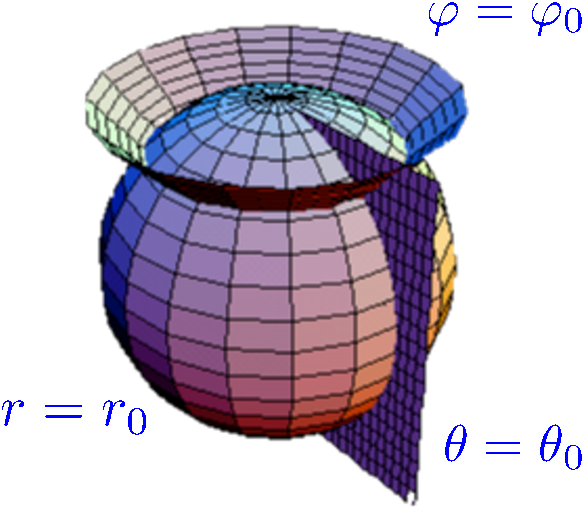
\includegraphics{./images/ch11/sphereP.pdf}}
\end{center}

球坐标系下的体积微元

\begin{center}
	\resizebox{!}{5.5cm}{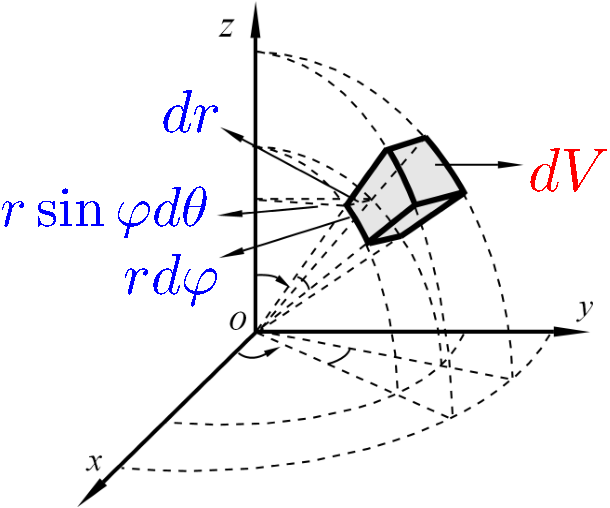
\includegraphics{./images/ch11/sphDv.pdf}} 
\end{center}

$$\d V=r^2\sin\varphi \d r\d\theta \d\varphi$$

{\bf P211-例7:}计算三重积分
$$\iiint_{\Omega}(x^2+y^2+z^2)\d V,$$
其中$\Omega$由$z=\sqrt{x^2+y^2}$与$x^2+y^2+z^2=R^2$所围成。

{\bf P212-例8:}计算三重积分
$$\iiint_{\Omega}(x^2+y^2)\d V,$$
其中$\Omega$由$x^2+y^2+z^2=2az$与$x^2+y^2+z^2=2bz$所围成$(0<a<b)$。

{\bf 注:}根据积分区域和被积函数的特点灵活选择坐标系

\section{重积分的应用}

\subsection{质量}

{P218-例1:}设一平面三角形薄片以$O(0,0),A(1,0),B(0,1)$为顶点,
其上任一点$(x,y)$处的面密度$\mu(x,y)=x^2+y^2$,
求该平面薄片的质量。

\subsection{质心(重心、形心)}

{\bf 空间$n$个质点的质心:}
	
空间中$n$个质点($k=1,2,\ldots,n$),质量分别为$m_k$,坐标$(x_k,y_k,z_k)$
$${\bar{x}=\df{\sum\limits_{k=1}^nx_km_k}{\sum\limits_{k=1}^nm_k},}\;
{\bar{y}=\df{\sum\limits_{k=1}^ny_km_k}{\sum\limits_{k=1}^nm_k},}\; 
{\bar{z}=\df{\sum\limits_{k=1}^nz_km_k}{\sum\limits_{k=1}^nm_k}}$$

{\bf 平面薄片的质心:} 密度函数$\mu(x,y)$,$(x,y)\in D$
$${\bar{x}=\df{\displaystyle\iint_Dx\mu(x,y)\d\sigma}
{\displaystyle\iint_D\mu(x,y)\d\sigma},\;} 
{\bar{y}=\df{\displaystyle\iint_Dy\mu(x,y)\d\sigma}
{\displaystyle\iint_D\mu(x,y)\d\sigma}}$$

{\bf P222-例2}
设半径为$R$的半圆形薄片上每一点的面密度与该点到圆心的距离成正比,
求该薄片的质心。

{\bb 空间物体的质心:} 密度函数$\mu(x,y,z)$,$(x,y,z)\in\Omega$
$$\bar{x}=\df{\displaystyle\iiint_{\Omega}x\mu(x,y,z)\d V}
{\displaystyle\iiint_{\Omega}\mu(x,y,z)\d V},\;
{\bar{y}=\df{\displaystyle\iiint_{\Omega}y\mu(x,y,z)dV}
{\displaystyle\iiint_{\Omega}\mu(x,y,z)dV},\;} $$
$${\bar{z}=\df{\displaystyle\iiint_{\Omega}z\mu(x,y,z)dV}
{\displaystyle\iiint_{\Omega}\mu(x,y,z)dV}}
$$
{\bf P223-例3:}求均匀半球壳$\Omega:a^2\leq x^2+y^2+z^2\leq b^2$
的形心。

\subsection{转动惯量}

{\bf 空间一质点的转动惯量:}$${I=mr^2}$$

\begin{center}
	\resizebox{!}{4cm}{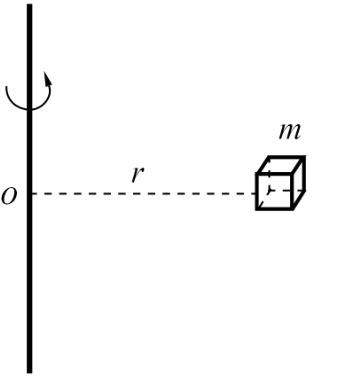
\includegraphics{./images/ch11/roll.pdf}}
\end{center}

{\bf 空间物体绕$z$轴旋转:}密度函数$\mu(x,y,z),(x,y,z)\in\Omega$
$${I=\iiint_{\Omega}(x^2+y^2)\mu(x,y,z)\d V}$$

{P225-例7:}求半径为$R$的均匀半圆形薄片绕其平分线转动的转动惯量和旋转半径。

{P225-例8:}(平行轴定理)设$L_c$为通过物体$\Omega$质心的直线,直线$L_t$平行于$L_c$,
两者距离为$d$。试证:$\Omega$关于轴$L_t$的转动惯量$I_t$与物体关于轴
$L_c$的转动惯量$I_c$之间存在关系如下:
$$I_t=I_c+Md\,^2,$$
其中$M$为$\Omega$的质量。

\subsection{万有引力}

物体$\Omega$的点密度为$\mu(x,y,z)$,质量为$m$的质点位于
$(a,b,c)$,$\Omega$对$m$的引力为:
$${F_x=\iiint_{\Omega}Km\mu\df{x-a}{r^3}\d V,} $$
$${F_y=\iiint_{\Omega}Km\mu\df{y-b}{r^3}\d V,} $$
$${F_z=\iiint_{\Omega}Km\mu\df{z-c}{r^3}\d V} $$

{\bf P227-例9:}求高为$H$,底半径为$R$且密度均匀的圆柱体,对其底面中心
一单位质量质点的引力。

\begin{center}
	\resizebox{!}{5cm}{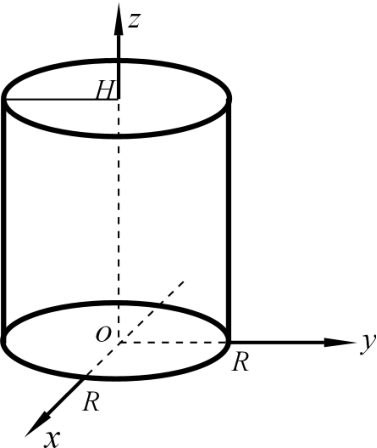
\includegraphics{./images/ch11/cg.pdf}}
\end{center}

\subsection{空间曲面的表面积}

已知函数$z=f(x,y)\,(x,y)\in D$,求其对应曲面的表面积。

$${S=\iint_D\sqrt{1+(f\,'_x)^2+(f\,'_y)^2}\d\sigma}$$

{\bf 例:}求半径为$a$的球的表面积。

\section{习题课}

\subsection{二重积分的计算}

{\bf 例:}计算下列二重积分
\begin{enumerate}[(1)]
  \setlength{\itemindent}{1cm}
  \item $\ds\iint_Dxye^{xy^2}\d\sigma,\,D=\{0\leq x\leq 1,0\leq
  y\leq 1\}$ 
  \item $\ds\iint_D\df 1{x+y}\d\sigma,\,D=\{0\leq x\leq 1,1\leq x+y\leq
  2\}$ 
  \item $\ds\iint_D|x^2+y^2-4|\d\sigma,\,D=\{x^2+y^2\leq 9\}$ 
  \item $\ds\iint_D(x+y)\mathrm{sgn}(x-y)\d\sigma,\,D=\{0\leq x\leq 1,0\leq
  y\leq 1\}$
\end{enumerate}

{\bf 例:}改变下列累次积分的次序
\begin{enumerate}[(1)]
  \setlength{\itemindent}{1cm}
  \item $\dint_0^1\dint_0^xf(x,y)\d
  y\d x+\dint_1^2\dint_0^{2-x}f(x,y)\d y\d x$
  \item $\dint_0^{2a}\dint_{\sqrt{2ax-x^2}}^{\sqrt{2ax}}
  f(x,y)\d y\d x,\;(a>0)$ 
  \item $\dint_0^{2\pi}\dint_0^{\sin x}f(x,y)\d y\d x$
\end{enumerate}

{\bf 例:}设$f(x)$在区间$[a,b]$连续且恒大于零,证明:
$$\dint_a^bf(x)\d x\dint_a^b\df{\d x}{f(x)}\geq (b-a)^2$$

{\bf 例:}利用二重积分的方法证明
$$\left[\dint_a^bf(x)g(x)\d x\right]^2\leq
\dint_a^bf\,^2(x)\d x\dint_a^bg^2(x)\d x$$

{\bf 例:}设$f(x)$在$[a,b]$上单调递增且恒为正,证明
$${\dint_0^1xf\,^2(x)\d x}{\dint_0^1f(x)\d x}\leq
{\dint_0^1f\,^2(x)\d x}{\dint_0^1xf(x)\d x}$$

\subsection{二重积分与坐标变换}

{\bf 例:}计算
$$\iint_{x^2+y^2\leq 1}\df{\d\sigma}{(x^2+y^2)^m}$$

{\bf 例:}设$f(x)$可微,$f(0)=0,\,f\,'(0)=1$,求
$$\lim\limits_{t\to 0^+}\df 1{\pi t^3}
\iint_{x^2+y^2\leq t^2}f\left(
\sqrt{x^2+y^2}\right)\d x\d y$$

{\bf 一般的积分坐标变换}

设$x=x(u,v),y=y(u,v)$为一一映射、一阶偏导连续且$\df{\p(x,y)}{\p(u,v)}\ne0$,则
$$\iint_Df(x,y)dxdy=\iint_D f(x,y)\left|\df{\p(x,y)}{\p(u,v)}\right|
\d u\d v$$

{\bf 注:}对于三重积分,有类似的公式成立!

{\bf 例:}通过适当的变量替换,将下列二重积分化为定积分 
\begin{enumerate}[(1)]
  \setlength{\itemindent}{1cm}
  \item $\ds\iint_{|x|+|y|\leq 1}f(x+y)\d\sigma$ 
  \item $\ds\iint_Df(xy)\d\sigma$,$D$由$xy=1,xy=2,y=x,y=4x,(x>0,y>0)$围成 
  \item $\ds\iint_{x^2+y^2\leq 1} f(ax+by+c)\d\sigma,\;(a^2+b^2\ne 0)$
\end{enumerate}

{\bf 例:}设$a^2+b^2=1,\, D:x^2+y^2\leq 1$,证明
$$\iint_Df(ax+by)\d x\d y=2\dint_{-1}^1f(u)\sqrt{1-u^2}\d u.$$

\subsection{三重积分的计算}

{\bf 例:}设$f(z)$连续,证明:
$$\iiint_{x^2+y^2+z^2\leq 1}f(z)\d V=\pi\dint_{-1}^1f(u)(1-u^2)\d u$$

{\bf 例:}计算三重积分
$$\iiint_{\Omega}z^2\d V,\;\Omega:x^2+y^2+z^2\leq 1,\,z\geq 0$$

{\bf 例:}按给定的积分次序重写累次积分
$$\dint_0^1\dint_0^x\dint_0^{xy}f(x,y,z)\d z\d y\d x$$
\begin{enumerate}[(1)]
  \setlength{\itemindent}{1cm}
  \item 先$y$后$z$后$x$
  \item 先$x$后$z$后$y$
\end{enumerate}

\begin{center}
	\resizebox{!}{5cm}{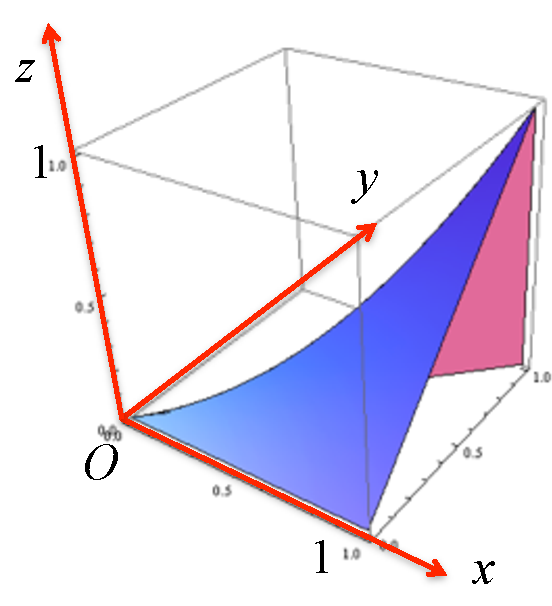
\includegraphics{./images/ch11/xyzC.pdf}}
\end{center}

\subsection{三重积分与坐标变换}

{\bf 例:}将三重积分
$$\dint_0^1\dint_{-\sqrt{y-y^2}}^{\sqrt{y-y^2}}
\dint_0^{\sqrt{3(x^2+3y^2)}}f\left(
\sqrt{x^2+y^2+z^2}\right)\d z\d x\d y$$
分别化为柱坐标和球坐标下的三重积分。

{\bf 例:}计算积分
$$\iiint_{\Omega}(x+y+z)^2\d V,$$
其中$\Omega:\;\df{x^2}{a^2}+\df{y^2}{b^2}+\df{z^2}{c^2}\leq 1$

{\bf 例:}计算由以下平面所围成的立体体积:
$$a_ix+b_iy+c_iz=\pm h_i,\;i=1,2,3,$$
其中:$a_i,b_i,c_i(i=1,2,3)$为常数,且
$$\Delta=\left|\begin{array}{ccc}
a_1 & b_1 & c_1\\ a_2 & b_2 & c_2 \\ a_3 & b_3 & c_3
\end{array}\right|\ne 0$$

{\bf 例:}计算极限
$$\lim\limits_{n\to\infty}\df 1{n^4}\iiint_{r\leq n}[r]\d V,$$
其中$r=\sqrt{x^2+y^2+z^2}$。

$${\df 43\pi\left[n^4-\sum\limits_{k=1}^nk^3\right]}$$

{\bf 例:}设$f(x)$可微,
$$F(t)=\iiint_{x^2+y^2+z^2\leq t^2}f(x^2+y^2+z^2)\d V,$$
求$F\,'(t)$。

{\bf 例:}设$f(x)$可微,
$$F(x)=\dint_0^x\d v\dint_0^v\d u\dint_0^uf(t)\d t,$$
求$F\,'(x)$。

\subsection{三重积分与坐标变换*}

求以下曲面在第一卦限中所围立体体积
$$\left(\df xa+\df yb\right)^2+\left(\df zc\right)^2=1,$$
其中$a,b,c>0$。

\subsection{重积分的应用}

{\bf 例:}在一半径为$R$的球内,以某条直径为轴打一个半径为$r(r<R)$的
圆孔,求打孔后球内剩余部分的体积。

{\bf 例:}求锥面$3(x^2+y^2)=(z-3)^2$与$z=0$所围的内切球面
与该锥面所围成的立体的体积。

\subsection{$n$重积分*}

{\bf 例:}求$n$维单纯形
$$T_n:\; x_i\geq 0\,(i=1,2,\ldots,n),\;
\sum\limits_{i=1}^nx_i\leq a$$
的体积$(a>0)$。\ps{单纯性是三角形在高维空间中的推广}

$$\df{a^n}{n!}$$

{\bf 例:}证明:
$$\dint_0^t\d t_1\dint_0^{t_1}\d t_2\ldots
\dint_0^{t_{n-1}}\prod\limits_{i=1}^nf(t_i)\d t_n
=\df 1{n!}\left[\dint_0^tf(s)\d s\right]^n$$

{\bf 例:}求$n$维单位球
$$\sum\limits_{k=1}^nx_k^2\leq 1$$
的体积。

$${\Gamma(\alpha)=\dint_0^{+\infty}x^{\alpha-1}e^{-x}dx,\;(\alpha>0)}$$

$${V_n=\df{2\pi^{n/2}}{n\Gamma(n/2)}}$$

\newpage

\section*{课后作业}

{\bf 【基本题】}

\begin{itemize}
  \setlength{\itemindent}{1cm}
  \item 习题11.1:1,7
  \item 习题11.2:1(3,4),3(1,3),6(2,3),9,10,13,15
  \item 习题11.3:1,4,12,16
  \item 习题11.4:1,2,4
\end{itemize}

{\bf 【上交题】}

\begin{itemize}
  \setlength{\itemindent}{1cm}
  \item 习题11.1:10
  \item 习题11.2:4(2,3),5,7(1),11,17,19,24
  \item 习题11.3:5(2),7,10,13,14,19
  \item 习题11.4:6,7,10,12,14,15,16
\end{itemize}

{\bf 【思考题】}

\begin{itemize}
  \setlength{\itemindent}{1cm}
  \item 习题11.2:7(2,3),12,16,22,25
  \item 习题11.3:15,18
\end{itemize}

\newpage

{\Large\bf 第11章习题课作业}

{\it (请抄题)}

\bigskip

1、改变下列累次积分的次序
\begin{enumerate}[(1)]
  \setlength{\itemindent}{1cm}
  \item $\dint_0^{2a}\dint_{\sqrt{2ax-x^2}}^{\sqrt{2ax}}
  f(x,y)\d y\d x,\;(a>0)$ 
  \item $\dint_0^{2\pi}\dint_0^{\sin x}f(x,y)\d y\d x$
\end{enumerate}

2、设$f(x)$在$[a,b]$上单调递增且恒非负,证明
$${\dint_a^b xf\,^2(x)\d x}{\dint_a^b f(x)\d x}\geq
{\dint_a^b f\,^2(x)\d x}{\dint_a^b xf(x)\d x}$$

3、设$f(x)$可微,$f(0)=0,\,f\,'(0)=1$,求
$$\lim\limits_{t\to 0^+}\df 1{\pi t^3}
\iint_{x^2+y^2\leq t^2}f\left(
\sqrt{x^2+y^2}\right)\d x\d y$$

4、计算二重积分$\ds\iint_D xy\d\sigma$,其中$D$由$xy=1,xy=2,y=x,y=4x$围成。 

5、设$f(z)$连续,证明:
$$\iiint_{x^2+y^2+z^2\leq 1}f(z)\d V=\pi\dint_{-1}^1f(u)(1-u^2)\d u$$

6、按先$x$后$z$后$y$的积分次序重写累次积分
$$\dint_0^1\dint_0^x\dint_0^{xy}f(x,y,z)\d z\d y\d x$$

7、计算积分
$$\iiint_{\Omega}(x+y+z)^2\d V,$$
其中$\Omega:\;\df{x^2}{a^2}+\df{y^2}{b^2}+\df{z^2}{c^2}\leq 1$。
\quad{\it (提示:由对称性,原式$=\ds\iiint_{\Omega}(x^2+y^2+z^2)\d V$)}

\bigskip

{\bf 以下题目选作:}

\bigskip

8、计算由以下平面所围成的立体体积:
$$a_ix+b_iy+c_iz=\pm h_i,\;i=1,2,3,$$
其中:$a_i,b_i,c_i(i=1,2,3)$为常数,且
$$\Delta=\left|\begin{array}{ccc}
a_1 & b_1 & c_1\\ a_2 & b_2 & c_2 \\ a_3 & b_3 & c_3
\end{array}\right|\ne 0$$

9、求$n$维单纯形$T_n:\; x_i\geq 0\,(i=1,2,\ldots,n),\;
\sum\limits_{i=1}^nx_i\leq a$
的体积$(a>0)$。

10、证明:
$$\dint_0^t\d t_1\dint_0^{t_1}\d t_2\ldots
\dint_0^{t_{n-1}}\prod\limits_{i=1}^nf(t_i)\d t_n
=\df 1{n!}\left[\dint_0^tf(s)\d s\right]^n$$

\newpage

{\bf 例:}求$n$维单位球的体积。

{\bf 解:}令
$$
\left\{
\begin{array}{l}
x_1=r\sin\theta_1\sin\theta_2\cdots\sin\theta_{n-2}\sin\theta_{n-1}\\
x_2=r\sin\theta_1\sin\theta_2\cdots\sin\theta_{n-2}\cos\theta_{n-1}\\
x_3=r\sin\theta_1\sin\theta_2\cdots\cos\theta_{n-2}\\
\cdots\hspace{1cm}\cdots\hspace{1cm}\cdots\\
x_{n-1}=r\sin\theta_1\cos\theta_2\\
x_n=r\cos\theta_1
\end{array}
\right..
$$
则$n$维单位球$S_n:\sum\limits_{i=1}^nx^2_i\leq1$可表示为
$$0\leq r\leq 1,\;(\theta_1,\theta_2,\ldots,\theta_{n-1})\in\Sigma_{n-1}.$$
又
$$J=\df{\p(x_1,x_2,\ldots,x_n)}{\p(r,\theta_1,\ldots,\theta_{n-1})}
=r^{n-1}\Delta_{n-1},$$
其中$\Delta_{n-1}$为某个关于$(\theta_1,\theta_2,\ldots,\theta_{n-1})$的函数,记
$$I_{n-1}=\dint\ldots\dint_{\Sigma_{n-1}}|\Delta_{n-1}|
\d\theta_1\ldots\d\theta_{n-1},$$
于是
$n$维单位球的体积
$$V_n=\dint\ldots\dint_{\Omega_n}\d V
=\dint_0^1\left[\dint\ldots\dint_{\Sigma_{n-1}}r^{n-1}|\Delta_{n-1}|
\d\theta_1\ldots\d\theta_{n-1}\right]\d r=\df1nI_{n-1}.$$

以下求$I_{n-1}$。注意到
$$\pi^{\frac n2}=\left(\dint_{-\infty}^{+\infty}e^{-x^2}\d x\right)^n
=\dint\ldots\dint_{\mathbb{R}^n}e^{-(x_1^2+\ldots+x_n^2)}\d V,$$
使用前述变换,$\mathbb{R}^n$可表示为
$$0\leq r<+\infty,
\;(\theta_1,\theta_2,\ldots,\theta_{n-1})\in\Sigma_{n-1}.$$
从而(注:$\Gamma(s)=\dint_0^{+\infty}e^{-x}x^{s-1}\d x$)
\begin{eqnarray*}
	\pi^{\frac n2}&=&\dint_0^{+\infty}
	\left[\dint\ldots\dint_{\Sigma_{n-1}}e^{-r^2}r^{n-1}|\Delta_{n-1}|
	\d\theta_1\ldots\ldots\d\theta_{n-1}\right]\d r\\
	&=&I_{n-1}\dint_0^{+\infty}e^{-r^2}r^{n-1}\d r
	=I_{n-1}\df{\Gamma\left(\df{n}2\right)}2.
\end{eqnarray*}
故
$$I_{n-1}=\df{2\pi^{\frac n2}}{\Gamma\left(\df{n}2\right)},$$
进而可得
$$V_n=\df{2\pi^{\frac n2}}{n\Gamma\left(\df{n}2\right)}.$$

{\bf 推论:}$\limn V_n=0$.

{\bf 证明:}注意到$\Gamma(s)=(s-1)\Gamma(s-1)$,取$N=[8\pi]+1$,则对$\forall n>N$有
$$\df{V_{n+2}}{V_n}=\df{2\pi(n+2)}{n^2}<\df12.$$
于是
$$0<V_n<\left(\df12\right)^{\left[\frac{n-N}2\right]}V_N,$$
显然$\left(\df12\right)^{\left[\frac{n-N}2\right]}V_N\to0(n\to\infty)$,利用夹逼定理,
即证。

\newpage

\begin{center}
	{\Large\bf 选择题测试}
	
	{\it (60分钟,每题3分,总分:99+1)}
\end{center}

\begin{enumerate}
  \item 设$x,e^x,e^{2x}$分别为方程$y''+p(x)y'+q(x)y=f(x)$的三个解,则
  该方程满足$y(0)=1,y'(0)=3$的特解为
  (\underline{\hspace{1cm}})
  %\ps{A}
  
  (A)$2e^{2x}-e^x$\hspace{1cm}(B)$e^x-2e^{2x}$ \hspace{1cm}
  (C)$e^{2x}-e^x$\hspace{1cm}(D)$2e^{2x}-\cos x$
%   \begin{enumerate}[(A)]
%     \item $2e^{2x}-e^x$
%     \item $e^x-2e^{2x}$
%     \item $e^{2x}-e^x$
%     \item $2e^{2x}-\cos x$
%   \end{enumerate}
  \item 方程$y''+y=x^2+1+\sin x$的特解可设为
  (\underline{\hspace{1cm}})
  %\ps{C}
  \begin{enumerate}[(A)]
    \item $y^*=ax^2+bx+c+x(A\sin x+B\cos x)$
    \item $y^*=x(ax^2+bx+c+A\sin x+B\cos x)$
    \item $y^*=ax^2+bx+c+A\sin x$
    \item $y^*=ax^2+bx+c+A\cos x$
  \end{enumerate}
  \item 二重极限$\lim\limits_{(x,y)\to(0,0)}\df{xy^2}{x^2+y^4}=$
  (\underline{\hspace{1cm}})
  %\ps{D}  
  
  (A) $0$\hspace{1cm}(B) $1$  \hspace{1cm}(C)$\df12$\hspace{1cm}(D)不存在
  \item 函数$f(x,y)=x^2-ay^2$($a$为常数)在$(0,0)$处(\underline{\hspace{1cm}})
  %\ps{D}
  
  (A) 不取极值\quad{1cm}(B)取极小值\quad (C)取极大值\quad
  (D)是否取极值取决于$a$的值
%   \begin{enumerate}[(A)]
%     \item 不取极值
%     \item 取极小值
%     \item 取极大值
%     \item 是否取极值取决于$a$的值
%   \end{enumerate}
  \item 函数$f(x,y)=\left\{\begin{array}{ll}
  0&,(x,y)=(0,0)\\
  \df{xy}{x^2+y^2}&,else
  \end{array}\right.$在原点处(\underline{\hspace{1cm}})
  %\ps{B}
  \begin{enumerate}[(A)]
    \item 连续且存在偏导数
    \item 不连续但存在偏导数
    \item 连续但不存在偏导数
    \item 不连续也不存在偏导数
  \end{enumerate}
  \item 函数$z=\sqrt{x^2+y^2}$在原点处 
  (\underline{\hspace{1cm}})
  %\ps{C}
  \begin{enumerate}[(A)]
    \item 偏导数和各方向的方向导数均存在
    \item 偏导数不存在,但各方向的方向导数均存在
    \item 偏导数和各方向的方向导数均不存在
    \item 偏导数存在,但某些方向的方向导数不存在
  \end{enumerate}
  \item 曲面$z=x+f(x-z)$的所有切平面都与某定直线
  (\underline{\hspace{1cm}})
  %\ps{B}
  
  (A) 垂直\hspace{1cm}(B) 平行  \hspace{1cm}(C)夹角为$\pi/4$\hspace{1cm}
  (D)夹角为$\pi/3$
%   \begin{enumerate}[(A)]
%     \item 垂直
%     \item 平行
%     \item 夹角为$\pi/4$
%     \item 夹角为$\pi/3$
%   \end{enumerate}
  \item 设$f(x,y)=(y-x^2)(y-x^4)$,$P(0,0),M(1,1)$,则(\underline{\hspace{1cm}})
%   \ps{B}
  \begin{enumerate}[(A)]
    \item $P,M$均为$f(x,y)$的极值点
    \item $P,M$均不是$f(x,y)$的极值点
    \item $P$为$f(x,y)$的极值点,$M$不是
    \item $M$为$f(x,y)$的极值点,$P$不是
  \end{enumerate}
  \item $x^2+y^2=1$时,$f(x,y)=(x^2+y^2)e^{-(x^2+y^2)}$ 
  (\underline{\hspace{1cm}})
%   \ps{B}
  
  (A)不取极值\hspace{1cm}(B)取极大值 \hspace{1cm}
  (C)取极小值\hspace{1cm}(D)取最大值
%   \begin{enumerate}[(A)]
%     \item 不取极值
%     \item 取极大值
%     \item 取极小值
%     \item 取最大值
%   \end{enumerate}
  \item $f(x,y)$在原点附近连续,$\lim\limits_{(x,y)\to(0,0)}
  \df{f(x,y)-|xy|}{(x^2+y^2)^2}=1$,则$f(x,y)$在原点
  (\underline{\hspace{1cm}})
%   \ps{C}
  
  (A)不取极值\hspace{1cm}(B)取极大值 \hspace{1cm}(C)取极小值\hspace{1cm}
  (D)不一定取极值
%   \begin{enumerate}[(A)]
%     \item 不取极值
%     \item 取极大值
%     \item 取极小值
%     \item 不一定取极值
%   \end{enumerate}
  \item $D$是顶点为$(1,0),(1,1),(2,0)$的三角区域,
  $I_k=\ds\iint_D[\ln(x+y)]^k\d\sigma$,则(\underline{\hspace{1cm}})
%   \ps{B}
  
  (A)$I_1<I_2<I_3$\quad(B)$I_1>I_2>I_3$\quad
  (C)$I_1<I_3<I_2$\quad(D)$I_3<I_1<I_2$
%   \begin{enumerate}[(A)]
%     \item $I_1<I_2<I_3$
%     \item $I_1>I_2>I_3$
%     \item $I_1<I_3<I_2$
%     \item $I_3<I_1<I_2$
%   \end{enumerate}
  \item 设$D_1:x+y\leq1,x\geq 0,y\geq0;\,D_2:|x|+|y|\leq1$,
  $I_j=\ds\iint_{D_j}e^{|x|+|y|}\d\sigma(j=1,2)$,则
  (\underline{\hspace{1cm}})
%   \ps{C}
  
  (A)$I_1=I_2$\hspace{1cm}(B)$2I_1=I_2$\hspace{1cm}
  (C)$4I_1=I_2$\hspace{1cm}(D)$I_1=4I_2$
%   \begin{enumerate}[(A)]
%     \item $I_1=I_2$
%     \item $2I_1=I_2$
%     \item $4I_1=I_2$
%     \item $I_1=4I_2$
%   \end{enumerate}
  \item 设$\ds\iint_{x^2+y^2\leq a^2}\sqrt{a^2-x^2-y^2}\d\sigma=\pi$,
  则$a=$(\underline{\hspace{1cm}})
%   \ps{D}
  
  (A)$1$\hspace{1cm}(B)$\sqrt[3]{\df12}$\hspace{1cm}
  (C)$\sqrt[3]{\df34}$\hspace{1cm}(D)$\sqrt[3]{\df32}$
%   \begin{enumerate}[(A)]
%     \item $1$
%     \item $\sqrt[3]{\df12}$
%     \item $\sqrt[3]{\df34}$
%     \item $\sqrt[3]{\df32}$
%   \end{enumerate}
  \item 设$\Omega$为$z\geq{\sqrt{x^2+y^2}}(z\geq0)$介于$z=1$和$z=2$之间
  的部分,则$\ds\iiint_{\Omega}f(x^2+y^2+z^2)\d V=$
  (\underline{\hspace{1cm}})
%   \ps{A}
  \begin{enumerate}[(A)]
    \item $\dint_1^2\dint_0^{2\pi}\dint_0^zf(r^2+z^2)r\d r\d\theta\d z$
    \item $\dint_0^{2\pi}\dint_1^2r\dint_0^1f(r^2+z^2)\d z\d r\d\theta$
    \item $\dint_0^{2\pi}\dint_0^{\frac{\pi}4}\dint_1^2
    f(r^2)r^2\sin\varphi\d r\d\varphi\d\theta$
    \item $\dint_0^{2\pi}\dint_{\frac{\pi}2}^{\frac{\pi}4}\dint_1^2
    f(r^2)r^2\sin\varphi\d r\d\varphi\d\theta$
  \end{enumerate}
  \item 设$\Gamma$为上半圆周$x^2+y^2=2x$从原点到$(1,1)$的部分,则
  $\dint_{\Gamma}P(x,y)\d x+Q(x,y)\d y=$(\underline{\hspace{1cm}})
%   \ps{C}
  \begin{enumerate}[(A)]
    \item $\dint_{\Gamma}\left[P(x,y)(x-1)+Q(x,y)\sqrt{2x-x^2}\right]\d s$
    \item $\dint_{\Gamma}\left[P(x,y)(1-x)-Q(x,y)\sqrt{2x-x^2}\right]\d s$
    \item $\dint_{\Gamma}\left[P(x,y)\sqrt{2x-x^2}+Q(x,y)(1-x)\right]\d s$
    \item $\dint_{\Gamma}\left[-P(x,y)\sqrt{2x-x^2}+Q(x,y)(x-1)\right]\d s$
  \end{enumerate}
  \item 设$f(x)$可微,$f(0)=1$,则$\lim\limits_{t\to0^+}\df1{\pi t^3}
  \ds\iint_{x^2+y^2\leq t^2}  f(\sqrt{x^2+y^2})\d x\d y=$ 
  (\underline{\hspace{1cm}})
%   \ps{C}
  
  (A)$0$\hspace{1cm}(B)$\df23f'(0)$\hspace{1cm}
  (C)$+\infty$\hspace{1cm}(D)不存在但也不是$\infty$
%   \begin{enumerate}[(A)]
%     \item $0$
%     \item $\df23f'(0)$
%     \item $+\infty$
%     \item 不存在但也不是$\infty$
%   \end{enumerate}
  \item 设$\Gamma$为$A(-1,0),B(-3,2)$和$C(3,0)$为顶点的三角形区域沿$ABCA$方向
  的封闭折线,则$\ds\oint_{\Gamma}(3x-y)\d x+(x-2y)\d y=$
  (\underline{\hspace{1cm}})
%   \ps{D}
  
  (A)$16$\hspace{1cm}(B)$-16$\hspace{1cm}
  (C)$8$\hspace{1cm}(D)$-8$
%   \begin{enumerate}[(A)]
%     \item $16$
%     \item $-16$
%     \item $8$
%     \item $-8$
%   \end{enumerate}
  \item 设$S$为单位球的外侧,$S_1$为其上半部分,则下列等式成立的是
  (\underline{\hspace{1cm}})
%   \ps{A}
  \begin{enumerate}[(A)]
    \item $\ds\iint_{S}|z|\d S=2\ds\iint_{S_1}|z|\d S$
    \item $\ds\iint_{S}|z|\d x\d y=2\ds\iint_{S_1}|z|\d x\d y$
    \item $\ds\iint_{S}|y|\d x\d y=2\ds\iint_{S_1}|y|\d x\d y$
    \item $\ds\iint_{S}|x|\d x\d y=2\ds\iint_{S_1}|x|\d x\d y$
  \end{enumerate}
  \item 设$S$为$z=\sqrt{x^2+y^2}$被$z=1$所截得的有限部分的外侧,则
  $\ds\iint_S x\d y\d z+y\d z\d x+(z^2-2z)\d x\d y=$
  (\underline{\hspace{1cm}})
%   \ps{D}
  
  (A)$-\df32\pi$\hspace{1cm}(B)$0$\hspace{1cm}
  (C)$\df{\pi}2$\hspace{1cm}(D)$\df32\pi$
%   \begin{enumerate}[(A)]
%     \item $-\df32\pi$
%     \item $0$
%     \item $\df{\pi}2$
%     \item $\df32\pi$
%   \end{enumerate}
  \item 设$L_1:\df{x^2}{4}+\df{y^2}{9}=1,L_2:\df{x^2}{9}+\df{y^2}{4}=1$,
  二者所围封闭区域分别为$D_1,D_2$,则下列正确的是
  (\underline{\hspace{1cm}})
%   \ps{C}
  \begin{enumerate}[(A)]
    \item $\dint_{L_1}(x+y^2)\d s=2\dint_{L_2}y^2\d s$
    \item $\dint_{L_1}(x^2+y)\d s=2\dint_{L_2}(x^2+y)\d s$
    \item $\ds\iint_{D_1}(x+y^3)\d\sigma=2\ds\iint_{D_2}(x+y^3)\d\sigma$
    \item $\ds\iint_{D_1}(x^2+y)\d\sigma=2\ds\iint_{D_2}(x^2+y)\d\sigma$
  \end{enumerate}
  \item $f(x,y)$偏导连续,曲线$L:f(x,y)=1$过第二象限的点$M$
  和第四象限的点$N$,$\Gamma$为$L$上从$M$到$N$的一段弧,则下列
  小于零的是
  (\underline{\hspace{1cm}})
%   \ps{B}
  \begin{enumerate}[(A)]
    \item $\dint_{\Gamma}f(x,y)\d x$
    \item $\dint_{\Gamma}f(x,y)\d y$
    \item $\ds\int_{\Gamma}f(x,y)\d s$
    \item $\ds\int_{\Gamma}f\,'_x(x,y)\d x+f\,'_y(x,y)\d y$
  \end{enumerate}
  \item 设曲面$S_1:x^2+y^2+z^2=1(z\geq
  0)$,$S_2$为$S_1$在第一卦限中的部分,
  则以下正确的是
  (\underline{\hspace{1cm}})
%   \ps{C}
  \begin{enumerate}[(A)]
    \item $\ds\iint_{S_1}x\d S=4\iint_{S_2}x\d S$
    \item $\ds\iint_{S_1}y\d S=4\iint_{S_2}x\d S$
    \item $\ds\iint_{S_1}z\d S=4\iint_{S_2}x\d S$
    \item $\ds\iint_{S_1}xyz\d S=4\iint_{S_2}xyz\d S$
  \end{enumerate}
  \item 设$f(r)$二阶连续可微,$r=\sqrt{x^2+y^2+z^2}$,
  若$\mathrm{div}(\bigtriangledown\,f(r))=0$,则$f(r)=$
  (\underline{\hspace{1cm}})
%   \ps{B}
  
  (A)$C_1r+C_2$\hspace{1cm}(B)$C_1/r+C_2$\hspace{1cm}
  (C)$C_1r^2+C_2$\hspace{1cm}(D)$C_1/r^2+C_2$
%   \begin{enumerate}[(A)]
%     \item $C_1r+C_2$
%     \item $C_1/r+C_2$
%     \item $C_1r^2+C_2$
%     \item $C_1/r^2+C_2$
%   \end{enumerate}
  以上$C_1,C_2$为任意常数
  \item 设$\Gamma$是从原点沿折线$y=1-|x-1|$至点$(2,0)$,则
  $\dint_{\Gamma}-y\d x+x\d y=$
  (\underline{\hspace{1cm}})
%   \ps{D}
  
  (A)$0$\hspace{1cm}(B)$-1$\hspace{1cm}
  (C)$2$\hspace{1cm}(D)$-2$
%   \begin{enumerate}[(A)]
%     \item 0
%     \item -1
%     \item 2
%     \item -2
%   \end{enumerate}
  \item 设$S$是三个坐标面与平面$x=a,y=b,z=c$(其中$a,b,c$均大于零)所围成的
  封闭曲面的外侧,则$\ds\oiint_S(x^2-yz)\d y\d z+(y^2-zx)\d z\d x
  +(z^2-xy)\d x\d y=$
  (\underline{\hspace{1cm}})
%   \ps{A}
  \begin{enumerate}[(A)]
    \item $abc(a+b+c)$
    \item $a^2b^2c^2(a+b+c)$
    \item $ab+ac+bc$
    \item $(a+b+c)^2$
  \end{enumerate}
  \item 若$(x^4+4xy^3)\d x+(ax^2y^2-5y^4)\d y$为全微分,则其原函数为
  (\underline{\hspace{1cm}})
%   \ps{C}
  \begin{enumerate}[(A)]
    \item $\df15x^5+3x^2y^2-y^5+C$
    \item $\df15x^5+4x^2y^2-5y^4+C$
    \item $\df15x^5+2x^2y^3-y^5+C$
    \item $\df15x^5+2x^2y^3-5y^4+C$
  \end{enumerate}
  \item 设$\sumn(-1)^n\df{(x-a)^n}n$在$x>0$时发散,在$x=0$处收敛,则$a=$
  (\underline{\hspace{1cm}})
%   \ps{B}
  
  (A)$1$\hspace{1cm}(B)$-1$\hspace{1cm}
  (C)$2$\hspace{1cm}(D)$-2$
%   \begin{enumerate}[(A)]
%     \item 1
%     \item -1
%     \item 2
%     \item -2
%   \end{enumerate}
  \item 设$\sumn a_n(x-1)^n$在$x=-1$处收敛,则它在$x=2$处
  (\underline{\hspace{1cm}})
%   \ps{B}
  
  (A)发散\hspace{1cm}(B)绝对收敛\hspace{1cm}
  (C)条件收敛\hspace{1cm}(D)敛散性与$a_n$有关
%   \begin{enumerate}[(A)]
%     \item 发散
%     \item 绝对收敛
%     \item 条件收敛
%     \item 敛散性与$a_n$有关
%   \end{enumerate}
  \item 设$\sumn a_nx^n$和$\sumn b_nx^n$收敛半径均为$R$,
  $\sumn(a_n+b_n)x^n$收敛半径为$R_1$,则
  (\underline{\hspace{1cm}})
%   \ps{C}
  
  (A)$R=R_1$\hspace{1cm}(B)$R>R_1$\hspace{1cm}
  (C)$R\leq R_1$\hspace{1cm}(D)$R\geq R_1$
  \item 若级数$\sumn a_n$条件收敛,则$\sumn na_n(x-1)^n$在$x=\sqrt3$和$x=3$分别
  (\underline{\hspace{1cm}})
%   \ps{B}
  
  (A)收敛,收敛\hspace{1cm}(B)收敛,发散\hspace{1cm}
  (C)发散,收敛\hspace{1cm}(D)发散,发散
%   \begin{enumerate}[(A)]
%     \item $R=R_1$
%     \item $R>R_1$
%     \item $R\leq R_1$
%     \item $R\geq R_1$
%   \end{enumerate}
  \item 设$f(x)=\left\{\begin{array}{ll}
  x&,x\in[0,1/2]\\ 2(1-x)&,x\in(1/2,1)
  \end{array}\right.$,$S(x)=\df{a_0}2+\sumn a_n\cos n\pi x,
  (x\in\mathbb{R})$,其中$a_n=2\dint_0^1f(x)\cos n\pi x\d x
  (n=0,1,2,\ldots)$,则$S\left(-\df52\right)=$
  (\underline{\hspace{1cm}})
%   \ps{A}
  
  (A)$\df34$\hspace{1cm}(B)$\df12$\hspace{1cm}
  (C)$-\df34$\hspace{1cm}(D)$-\df12$
%   \begin{enumerate}[(A)]
%     \item $\df34$
%     \item $\df12$
%     \item $-\df34$
%     \item $-\df12$
%   \end{enumerate}
  \item 将函数$f(x)=\left\{\begin{array}{ll}
  1&,0\leq x<1\\ x+1&,1\leq x\leq \pi
  \end{array}\right.$在$[0,\pi]$上展开成余弦级数,则其和函数在$x=1$和$x=\pi$
  处的值分别为
  (\underline{\hspace{1cm}})
%   \ps{A}
  
  (A)$\df32,\pi+1$\hspace{1cm}(B) $2,0$\hspace{1cm}
  (C)$2,\pi+1$\hspace{1cm}(D)$\df32,\df{\pi}2+1$
%   \begin{enumerate}[(A)]
%     \item $\df32,\pi+1$
%     \item $2,0$
%     \item $2,\pi+1$
%     \item $\df32,\df{\pi}2+1$
%   \end{enumerate}
  \item 设$f(x)$连续,则$\dint_0^1\d y\dint_{-\sqrt{1-y^2}}^{1-y}f(x,y)\d y=$
  (\underline{\hspace{1cm}})
%   \ps{D}
  \begin{enumerate}[(A)]
    \item $\dint_0^1\d x\dint_{0}^{x-1}f(x,y)\d y
    +\dint_{-1}^0\d x\dint_0^{\sqrt{1-x^2}}f(x,y)\d y$
    \item $\dint_0^1\d x\dint_{0}^{1-x}f(x,y)\d y
    +\dint_{-1}^0\d x\dint_{-\sqrt{1-x^2}^0}f(x,y)\d y$
    \item $\dint_0^{\frac{\pi}2}\d\theta\dint_0^{\frac1{\cos\theta+\sin\theta}}
    f(r\cos\theta,f\sin\theta)\d r+\dint_{\frac{\pi}2}^{\pi}\d\theta
    \dint_0^{\frac1{\cos\theta+\sin\theta}}f(r\cos\theta,f\sin\theta)\d r$
    \item $\dint_0^{\frac{\pi}2}\d\theta\dint_0^{\frac1{\cos\theta+\sin\theta}}
    f(r\cos\theta,f\sin\theta)r\d r+\dint_{\frac{\pi}2}^{\pi}\d\theta
    \dint_0^{\frac1{\cos\theta+\sin\theta}}f(r\cos\theta,f\sin\theta)r\d r$
  \end{enumerate}
  
\end{enumerate}